%!TEX program = lualatex
\documentclass[spanish]{report}
\usepackage[T1]{fontenc}
\usepackage[spanish, es-lcroman]{babel}
\usepackage{geometry}
\usepackage{fontspec}
\usepackage{graphicx}
\usepackage[explicit]{titlesec}
\usepackage{hyperref}
\usepackage{float}
\usepackage{titletoc}
%\usepackage[titles]{tocloft}
\usepackage[backend=biber,style=apa]{biblatex}
\bibliography{Bibliografía}

\setmainfont{Arial}
\geometry{
	letterpaper,
	top=25mm,
	bottom=25mm,
	left=30mm,
	right=30mm
}

%%%%%%%%%%%%%%%%%%%%%%
\hyphenpenalty=10000
\tolerance=9999
%%%%%%%%%%%%%%%%%%%%%%

\setlength{\parindent}{0pt}
\setlength{\parskip}{2ex}

\titleformat{\chapter}[block]
{\bfseries\centering\fontsize{14pt}{2em}\fontspec{Arial}\selectfont}{
	\MakeUppercase{\chaptertitlename} \thechapter\\
}{0mm}{\MakeUppercase{#1}}


\renewcommand{\thechapter}{\Roman{chapter}}
\renewcommand{\thesection}{\arabic{chapter}.\arabic{section}}

\renewcommand{\thefigure}{\arabic{chapter}.\arabic{figure}}

\titlespacing*{\chapter}{0mm}{0mm}{10mm}


\begin{document}
	\newgeometry{margin=0in}
\begin{titlepage}
	\begin{picture}(-5,0)(2.5,0)
		\put(42.75,-741.5){
			\includegraphics[width=56.15001pt,height=57pt]{Imagenes/LogoItl.png}}
		\put(27.55,-93.45004){
			
\includegraphics[width=519.5pt,height=70.85pt]{Imagenes/LogoTecnm.png}}
	\end{picture}\par
	\centering
	\begin{minipage}{180mm}
		\vspace{40mm}
		\centering
		{\fontsize{18}{22pt}\selectfont\fontspec{Montserrat}
			\textbf{DEDEPARTAMENTO DE\\SISTEMAS Y COMPUTACIÓN}\par
		}
		\vspace{10mm}
		{\fontsize{15}{23pt}\selectfont\fontspec{Montserrat}
			\textbf{MATERIA}\par
			\vspace{9mm}
			\textbf{DESARROLLO DE APLICACIONES EMPRESARIALES}\par
		}
		\vspace{10mm}
		{\fontsize{17}{21pt}\selectfont\fontspec{Adobe Caslon Pro}
			REPORTE DE PROYECTO\par
		}
		\vspace{10mm}
		{\fontsize{14}{18pt}\selectfont\fontspec{Montserrat}
			\uppercase{
				Aplicación Registro de Asistentes a Congreso
			}
			\par
		}
		\vspace{10mm}
		{\fontsize{14}{18pt}\selectfont\fontspec{Montserrat}
			\textbf{
				P R E S E N T A N:
			}\par
		}
		\vspace{10mm}
		{\fontsize{14}{20pt}\selectfont\fontspec{Montserrat}
			\uppercase{\textbf{
				José Manuel Gómez García\\
				Armando Abraham Medina Delgado\\
				Aldair Rivaldo Sanita Leon\\
				Osvaldo Emmanuel Ruiz Veloz\\
				Fabrizio Moreno Mejía
			}}\par
		}
		\vspace{10mm}
		{\fontsize{14}{18pt}\selectfont\fontspec{Montserrat}
			\textbf{
				MAESTRO:
			}\par
		}
		\vspace{5mm}
		{\fontsize{12}{16pt}\selectfont\fontspec{Montserrat}
			\textbf{
				M.C. ISMAEL PÉREZ MENA
			}\par
		}
		\vspace{12mm}
		{\fontsize{10}{14pt}\selectfont\fontspec{Montserrat ExtraBold}
			LEÓN, GUANAJUATO. \hspace{70mm} 27 de noviembre del 2023\par
			%\today%21 de noviembre del 2023
		}
	\end{minipage}
\end{titlepage}
\restoregeometry
	\fontsize{12pt}{2em}\selectfont
	
	\tableofcontents
	\addcontentsline{toc}{chapter}{ÍNDICE GENERAL}
	\listoffigures
	\addcontentsline{toc}{chapter}{ÍNDICE DE FIGURAS}
	\input{Introducción}
	\input{Desarrollo de la Arquitectura de la Información}
	\chapter{Requerimientos del Proyecto}

\newcounter{cRequerimientos}
\setcounter{cRequerimientos}{0}
\newcommand{\IncReq}{\addtocounter{cRequerimientos}{1}}


\section{Funcionales}
\begin{list}{RF\_\IncReq\thecRequerimientos}{}
	\item Pantalla de registro de participantes que contenga un formulario para poder registrar un nuevo participante, guardando los siguientes datos: Nombre, Apellidos, Email, Usuario en Twitter, Avatar y una casilla para aceptar términos y condiciones.
	
	Al hacer clic en Guardar deberá de redirigirnos de nuevo al listado de participantes.
	
	\item Edición  de los datos de un participante.  Al hacer clic sobre el avatar la aplicación deberá de redirigir 
	a una pantalla donde se podrán editar los datos de un participante
\end{list}

\section{No Funcionales}

\begin{list}{RNF\_\IncReq\thecRequerimientos}{}
	\item En la pantalla de inicio se presentará una landing page con:
	\begin{itemize}
		\item El logotipo de la institución
		\item el nombre y el logotipo del congreso
		\item Un botón de acceso ``Entrar'' que hacer clic en él deberá de redirigir al listado de participantes.
	\end{itemize}
	
	\item En la pantalla de listado de participantes se deberá de mostrar un listado de cada uno de los Participantes que ya están registrados. 
	
	Cada participante se deberá mostrar en una tarjeta en la que aparecerá su nombre completo, enlace a su página de Twitter, ocupación y una imagen tipo avatar.
	(Se deberán utilizar tarjetas para generar el listado, no utilizar tablas)
\end{list}
	\chapter{Desarrollo de Diagramas UML}

\begin{figure}[H]
	\centering
	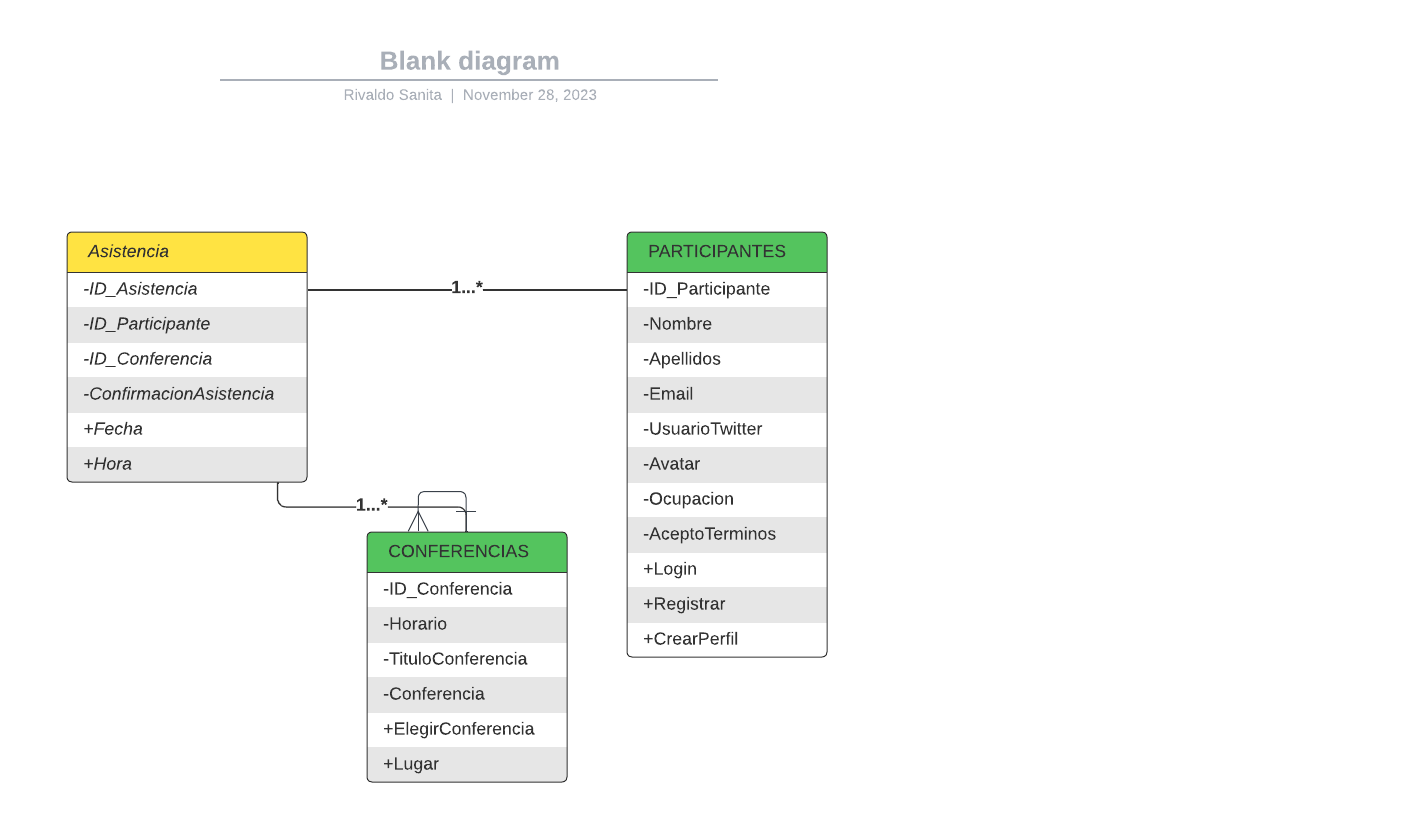
\includegraphics[width=1\linewidth]{Imagenes/Diagramas/UML}
	\caption{Diagrama UML de Clase}
	\label{fig:uml}
\end{figure}

\begin{figure}[H]
	\centering
	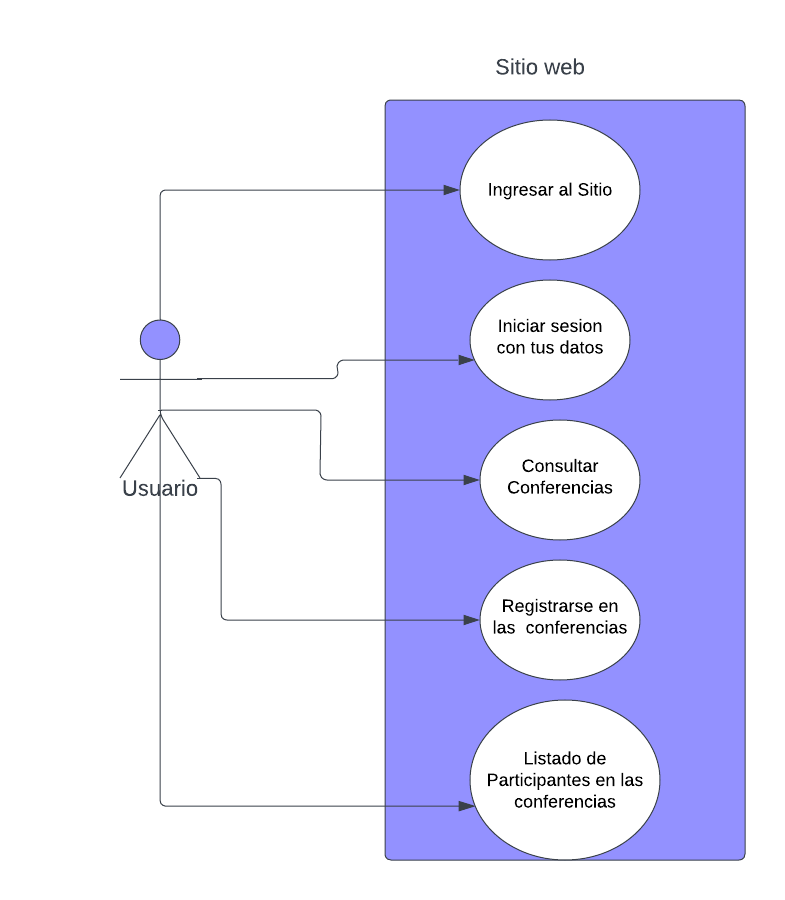
\includegraphics[width=0.9\linewidth]{Imagenes/Diagramas/Casos de uso}
	\caption{Diagrama de Casos de Uso}
	\label{fig:casos-de-uso}
\end{figure}


\begin{figure}[H]
	\centering
	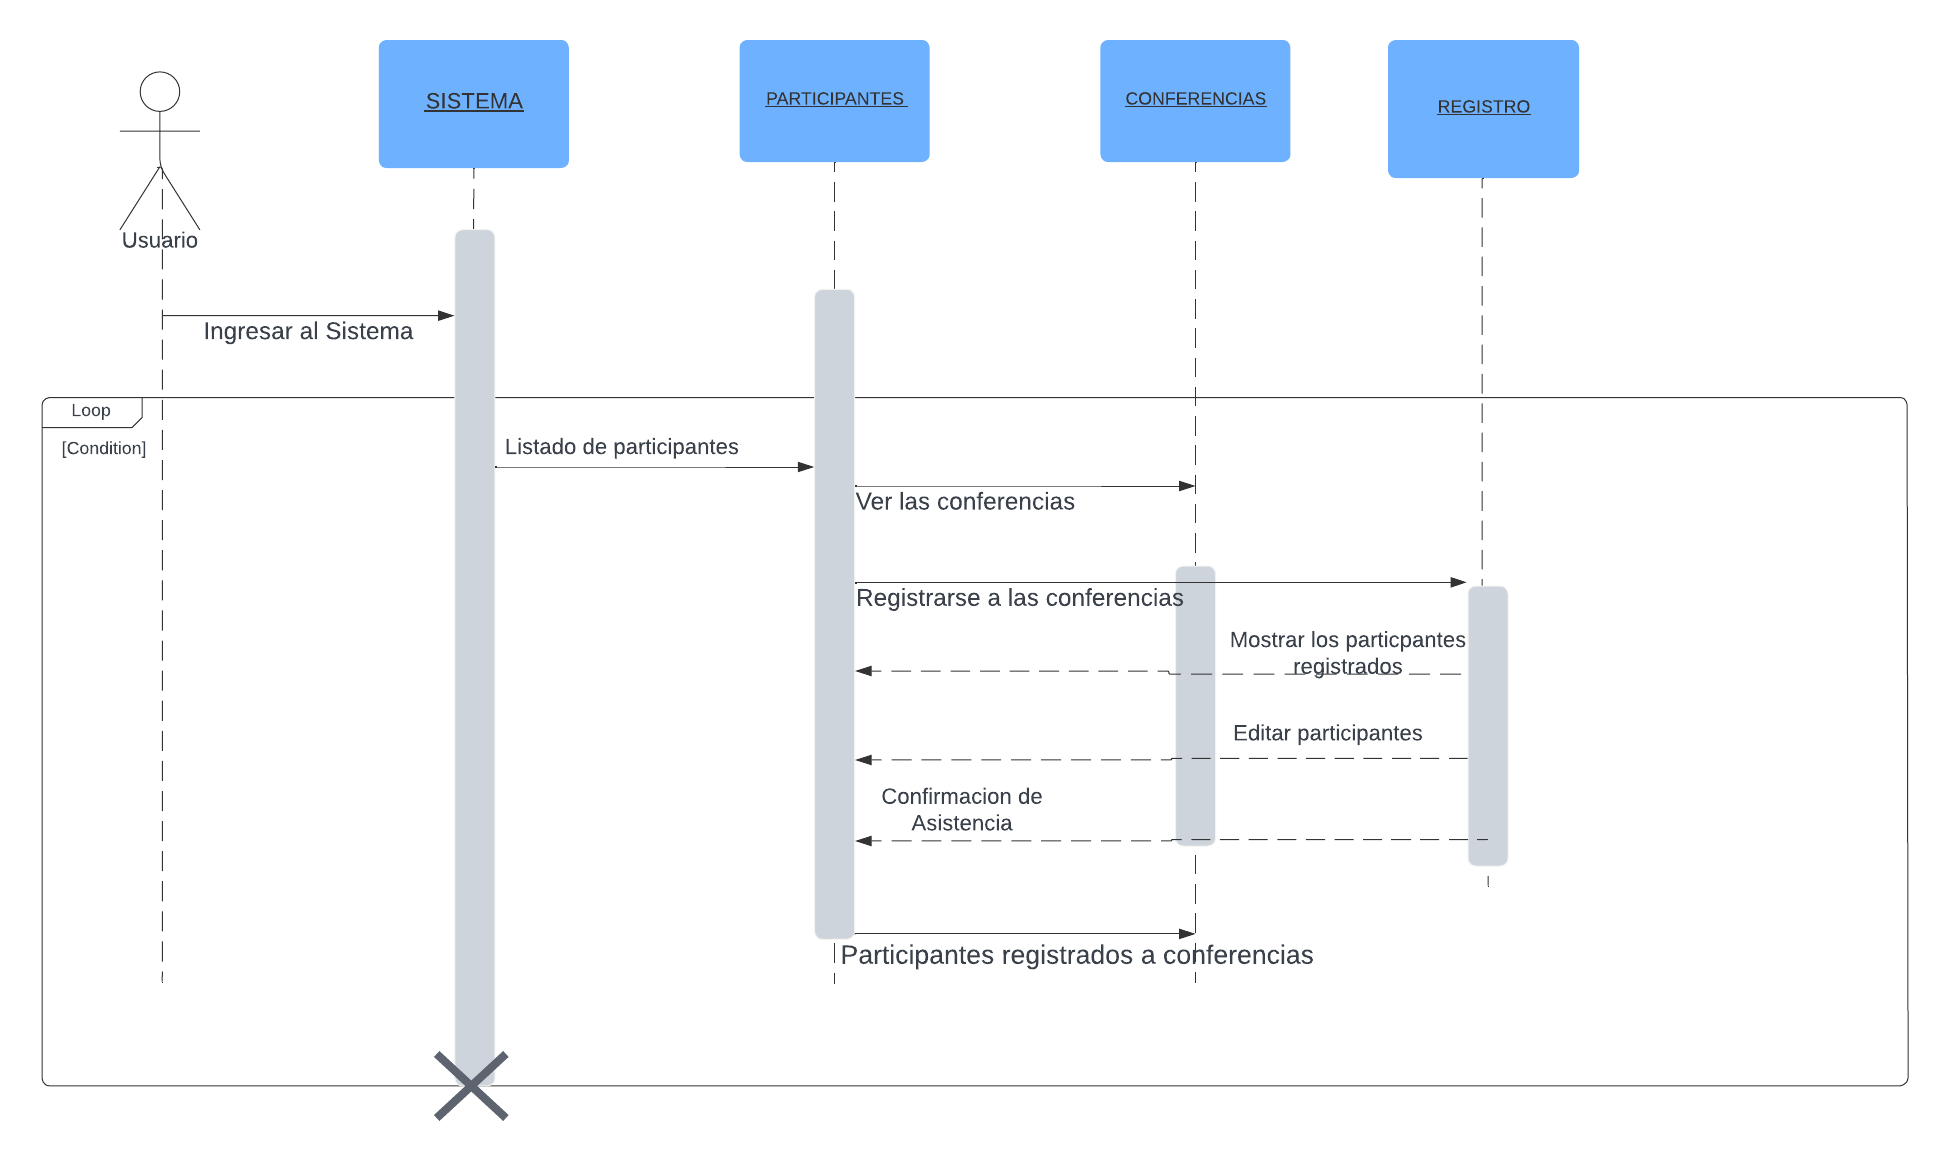
\includegraphics[width=1\linewidth]{Imagenes/Diagramas/Secuencia}
	\caption{Diagrama de Secuencia}
	\label{fig:secuencia}
\end{figure}






	\chapter{Diagramas de BD}
	\chapter*{CONCLUSIONES GENERALES} \addcontentsline{toc}{chapter}{CONCLUSIONES GENERALES}
{
	\fontsize{12pt}{10mm}\selectfont
	\begin{enumerate}
		\item Las aplicaciones Web son valiosas herramientas que se pueden utilizar para facilitar el trabajo de las empresas.
		\vspace{6mm}
		
		\item Actualmente gran parte de las empresas ya utilizan aplicaciones web en el desarrollo de sus procesos.
		\vspace{6mm}
		
		\item El poseer los conocimientos necesarios para el desarrollo de aplicaciones web, nos hará más competitivos en el mercado laboral.
		\vspace{6mm}
		
		\item A través de este trabajo hemos tenido que incursionar en muchos de los aspectos que involucra el desarrollo de aplicaciones web, lo cual está aportando valiosos conocimientos y capacidades para nuestra formación profesional.
		\vspace{6mm}
		
		\item El trabajo realizado nos sirvió de experiencia para llevar acabo trabajos o proyectos más involucrados al desarrollo web y asimismo tener experiencia para futuros proyectos.   
  
		\vspace{6mm}
	\end{enumerate}
}

	
	\nocite{*}
	\printbibliography
\end{document}